% ============================================================
\section{CUADRÚPEDO: SALTO}
% ============================================================

\begin{frame}{P1: Modelo Dinámico del Cuadrúpedo (SRBM)}
\begin{columns}[T]
\begin{column}{0.50\textwidth}
\begin{tbox}{Estado y Entradas}
\footnotesize
\textbf{Estado} $\bx \in \RR^{12}$ y \textbf{Control} $\bu \in \RR^{12}$:
\begin{align*}
\bx &= \begin{bmatrix}\bp\tr & \bm{\eta}\tr & \bv\tr & {}^b\bomega\tr\end{bmatrix}\tr\\
\bu &= \begin{bmatrix}\bef_{FR}\tr & \bef_{FL}\tr & \bef_{RR}\tr & \bef_{RL}\tr\end{bmatrix}\tr
\end{align*}
\begin{itemize}
\item $\bp=(x,y,z)$: posición del CdM en $\{W\}$.
\item $\bm{\eta}=(\phi,\theta,\psi)$: orientación roll--pitch--yaw.
\item $\bef_i$: fuerza de contacto del suelo sobre el pie $i$.
\end{itemize}
\end{tbox}
\end{column}

\begin{column}{0.46\textwidth}
\begin{tbox}{Ecuaciones de Movimiento}
\footnotesize
\begin{align*}
\dot{\bp} &= \bv \\
\dot{\bv} &= \mathbf{g} + \frac{1}{m}\sum_{i=1}^4 \bef_i \\
\dot{\bm{\eta}} &= E(\phi,\theta)\,{}^b\bomega \\
I\,{}^b\dot{\bomega} &= {}^w\bR_b\tr \sum_{i=1}^4 (\bp_i - \bp)\times \bef_i - {}^b\bomega \times (I\,{}^b\bomega)
\end{align*}
Patas modeladas sin masa (SRBM); parámetros leídos directamente del URDF del Go2.
\end{tbox}
\end{column}
\end{columns}
\src{Cinemática rotacional con matriz $E(\phi,\theta)$ y orientación $\bR = \bR_z(\psi)\bR_y(\theta)\bR_x(\phi)$}
\end{frame}

\begin{frame}{P1: Secuencia de Fases y Contactos}
\begin{columns}[T]
\begin{column}{0.48\textwidth}
\begin{tbox}{Estructura de 5 Fases ($N=88$ nodos)}
\scriptsize
\resizebox{\linewidth}{!}{%
\begin{tabular}{@{}clccc@{}}
\toprule
$j$ & Descripción & Apoyos $\mathcal{S}_j$ & $N_j$ & $T_j$ (s) \\
\midrule
1 & Impulso 4 patas & FR, FL, RR, RL & 22 & $[0.25,\,0.80]$ \\
2 & Impulso traseras & RR, RL & 10 & $[0.05,\,0.15]$ \\
3 & Vuelo libre & $\emptyset$ & 24 & $[0.15,\,1.70]$ \\
4 & Aterrizaje delanteras & FR, FL & 10 & $[0.05,\,0.15]$ \\
5 & Apoyo 4 patas & FR, FL, RR, RL & 22 & $[0.25,\,0.80]$ \\
\bottomrule
\end{tabular}}
\vskip4pt
Las duraciones $T_j$ son variables de decisión acotadas: $h_k = T_{j(k)}/N_{j(k)}$.
\end{tbox}
\end{column}

\begin{column}{0.48\textwidth}
\begin{tbox}{Restricciones Físicas de Contacto}
\small
\begin{itemize}
\item \textbf{Fricción y fuerza normal:}
\begin{gather*}
0 \le f_{z,i} \le 220\,\text{N}\\
|f_{x,i}| \le \mu f_{z,i},\quad |f_{y,i}| \le \mu f_{z,i}
\end{gather*}
con coeficiente de fricción $\mu = 0.70$.
\item \textbf{Pata en vuelo:} $\bef_i = \mathbf{0}$ si $i \notin \mathcal{S}_{j(k)}$.
\item \textbf{Alcance de pata:} $0.20 \le \|\bd_i\| \le 0.39$\,m, donde $\bd_i$ es el vector cadera--pie en $\{B\}$.
\end{itemize}
\end{tbox}
\end{column}
\end{columns}
\end{frame}

\begin{frame}{P1: Obstáculo Suave y Optimización NLP}
\begin{columns}[T]
\begin{column}{0.48\textwidth}
\begin{tbox}{Obstáculo Diferenciable}
\small
Caja de $H=0.25$\,m en $x \in [0.42, 0.67]$\,m aproximada mediante producto de sigmoides:
\begin{equation*}
\begin{aligned}
h_{\mathrm{obs}}(x) = (H+\delta)\,&\sigma\big(k(x-x_1+\delta)\big)\\
\cdot\,&\sigma\big(k(x_2+\delta-x)\big)
\end{aligned}
\end{equation*}
\begin{itemize}
\item Margen de inflado: $\delta = 3$\,cm, $k=80$.
\item Se exige $z_c \ge h_{\mathrm{obs}}(x_c)$ para esquinas del tronco, rodillas y pies durante todo el salto.
\end{itemize}
\end{tbox}
\end{column}

\begin{column}{0.48\textwidth}
\begin{tbox}{Problema NLP y Costo}
\small
\begin{equation*}
J = \sum_{k=0}^{N-1} h_k \ell_k + 0.02 \sum_{k=1}^{N-1} \Big\|\frac{\Delta \bu_k}{mg}\Big\|^2
\end{equation*}
\begin{equation*}
\ell_k = \Big\|\frac{\bu_k - \bu_k^{\mathrm{est}}}{mg}\Big\|^2 + 0.05\|{}^b\bomega_k\|^2 + 2(\phi_k^2 + \psi_k^2)
\end{equation*}
\begin{itemize}
\item Penaliza desviación del apoyo estático $\bu_k^{\mathrm{est}}$.
\item Regulariza variación temporal de fuerzas.
\end{itemize}
\end{tbox}
\end{column}
\end{columns}
\end{frame}

\begin{frame}{P1: Cinemática Inversa y Torques Articulares}
\begin{columns}[T]
\begin{column}{0.48\textwidth}
\begin{tbox}{Cinemática Inversa Analítica}
\small
Para cada pata $i$ ($q_0$: abducción, $q_1$: cadera, $q_2$: rodilla):
\begin{itemize}
\item \textbf{En apoyo:} posición del pie fija en el suelo:
\begin{equation*}
\bm{q}_i = \mathrm{CI}_i\big({}^w\bR_b\tr(\bp_i^c - \bp)\big)
\end{equation*}
\item \textbf{En vuelo:} interpolación quíntica articular suave entre despegue, pose recogida y aterrizaje.
\end{itemize}
\end{tbox}
\end{column}

\begin{column}{0.48\textwidth}
\begin{tbox}{Mapeo a Torques de Motores}
\small
Los torques requeridos en los motores para producir las fuerzas óptimas de contacto se obtienen con el \textbf{Jacobiano}:
\begin{equation*}
\btau_i = -J_i(\bm{q}_i)\tr\,{}^w\bR_b\tr\,\bef_i
\end{equation*}
\begin{itemize}
\item Permite validar que los actuadores no superen los límites de torque máximo.
\end{itemize}
\end{tbox}
\end{column}
\end{columns}
\end{frame}

\begin{frame}{P1: Resultados -- Secuencia del Salto}
\begin{center}
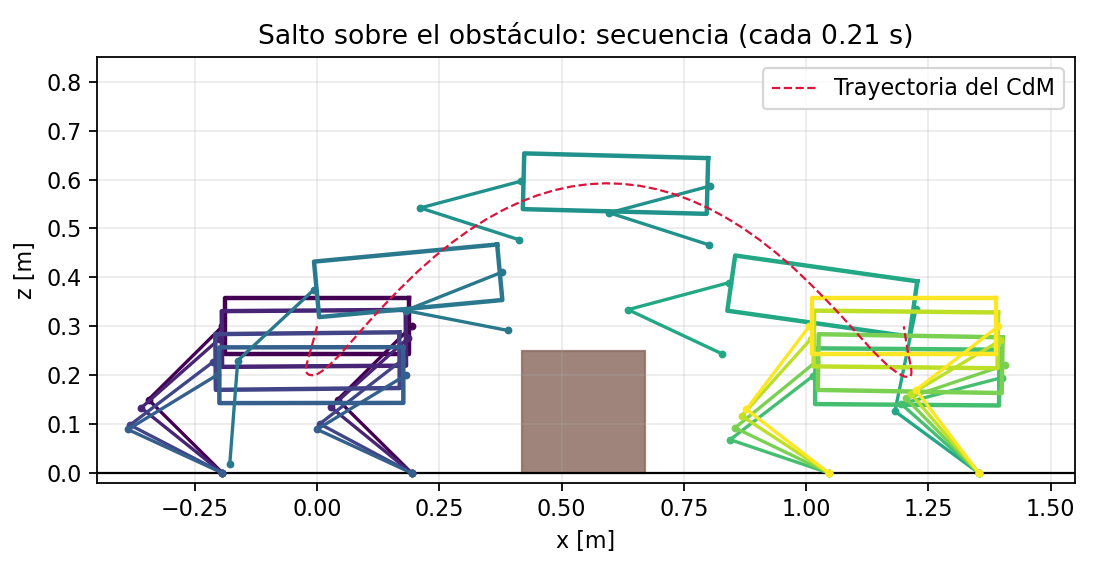
\includegraphics[width=0.56\textwidth]{p1_secuencia.png}
\end{center}
\begin{tbox}{Dinámica del Salto Observada}
\scriptsize
\begin{itemize}
\item \textbf{Fase 1 (Agachado):} El CdM desciende hasta $\approx 0.20$\,m acumulando energía.
\item \textbf{Fase 2 (Despegue):} Impulso con patas traseras; despegue con $v_x \approx 2$\,m/s, $v_z \approx 2$\,m/s.
\item \textbf{Fase 3 (Vuelo):} Ápice a $z_{\max} \approx 0.59$\,m, patas recogidas superando ampliamente el obstáculo de $0.25$\,m.
\item \textbf{Fases 4-5 (Aterrizaje):} Contacto secuencial (delanteras $\to$ traseras), frenado y estabilización en $x_f=1.20$\,m.
\end{itemize}
\end{tbox}
\end{frame}

\begin{frame}{P1: Resultados -- Estados del Cuerpo Rígido}
\begin{columns}[c]
\begin{column}{0.58\textwidth}
\centering
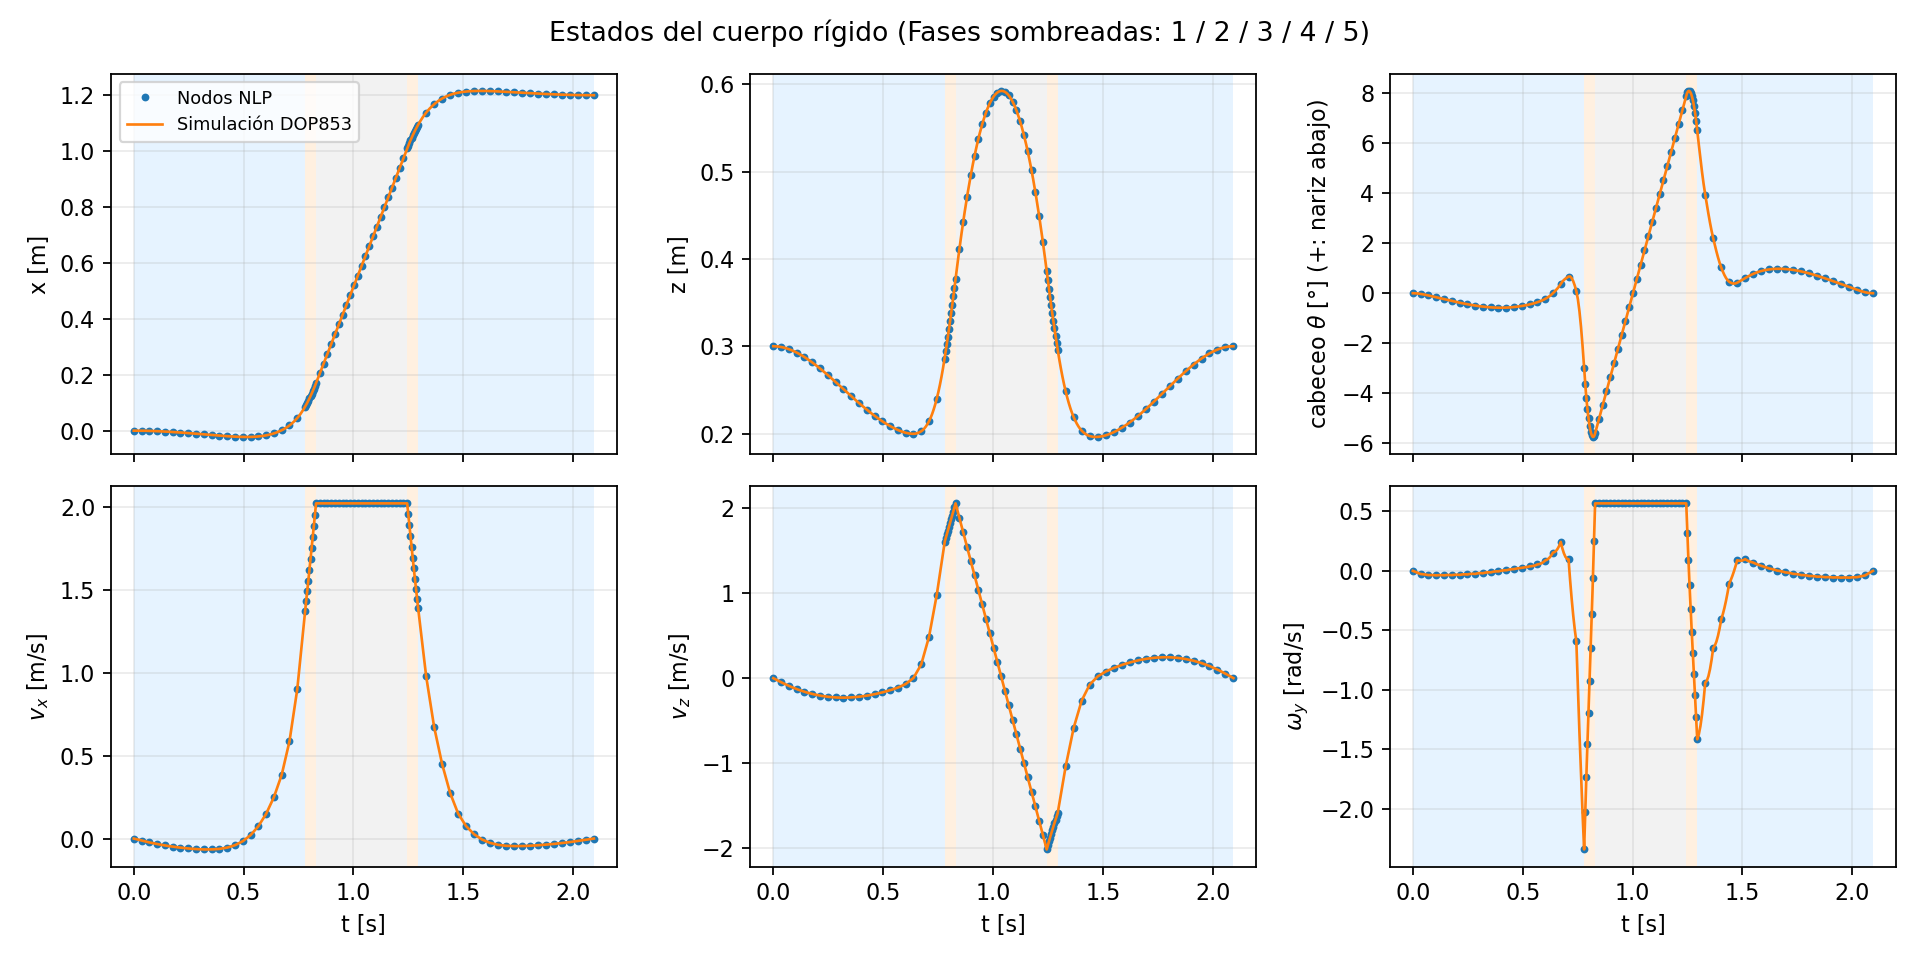
\includegraphics[width=\linewidth]{p1_estados.png}
\end{column}
\begin{column}{0.38\textwidth}
\begin{tbox}{Evolución Temporal}
\scriptsize
\begin{itemize}
\item Las 5 fases se distinguen por las bandas sombreadas.
\item El cabeceo $\theta$ (pitch) rota hacia arriba en el impulso y se nivela suavemente para el aterrizaje.
\item Roll ($\phi$) y Yaw ($\psi$) se mantienen cercanos a cero por la fuerte penalización y simetría.
\item Duración total optimizada: $\approx 2.1$\,s.
\end{itemize}
\end{tbox}
\end{column}
\end{columns}
\src{Animaciones: \href{https://github.com/LEKamt/rav_ec3/blob/7780e7d0c8741acd9c4335f4ed9dffac1bd24fd3/report/figures/p1_salto.gif}{p1\_salto.gif} y \href{https://github.com/LEKamt/rav_ec3/blob/7780e7d0c8741acd9c4335f4ed9dffac1bd24fd3/report/figures/p1_salto_slow.gif}{p1\_salto\_slow.gif} \\ \vspace{0.5cm}}
\end{frame}
